
% Classical Game chapter ----------------------------------------------
\chapter*{Classical Game}
\addcontentsline{toc}{chapter}{Classical Game}

\begin{flushright}
\parbox{0.8\textwidth}{
\emph{A great war leaves the country with three armies -
an army of cripples, an army of mourners, and an army of thieves. \\
\hspace*{\fill}{\textperiodcentered \textperiodcentered \textperiodcentered \hspace*{0.2em} German proverb} } }
\end{flushright}

\noindent
About classical chess is written really everything already, and I
have nothing to add. Except for illustration of initial setup, so that
you can accustom yourself with rendition of pieces used in this text.

\noindent
\begin{figure}[t]
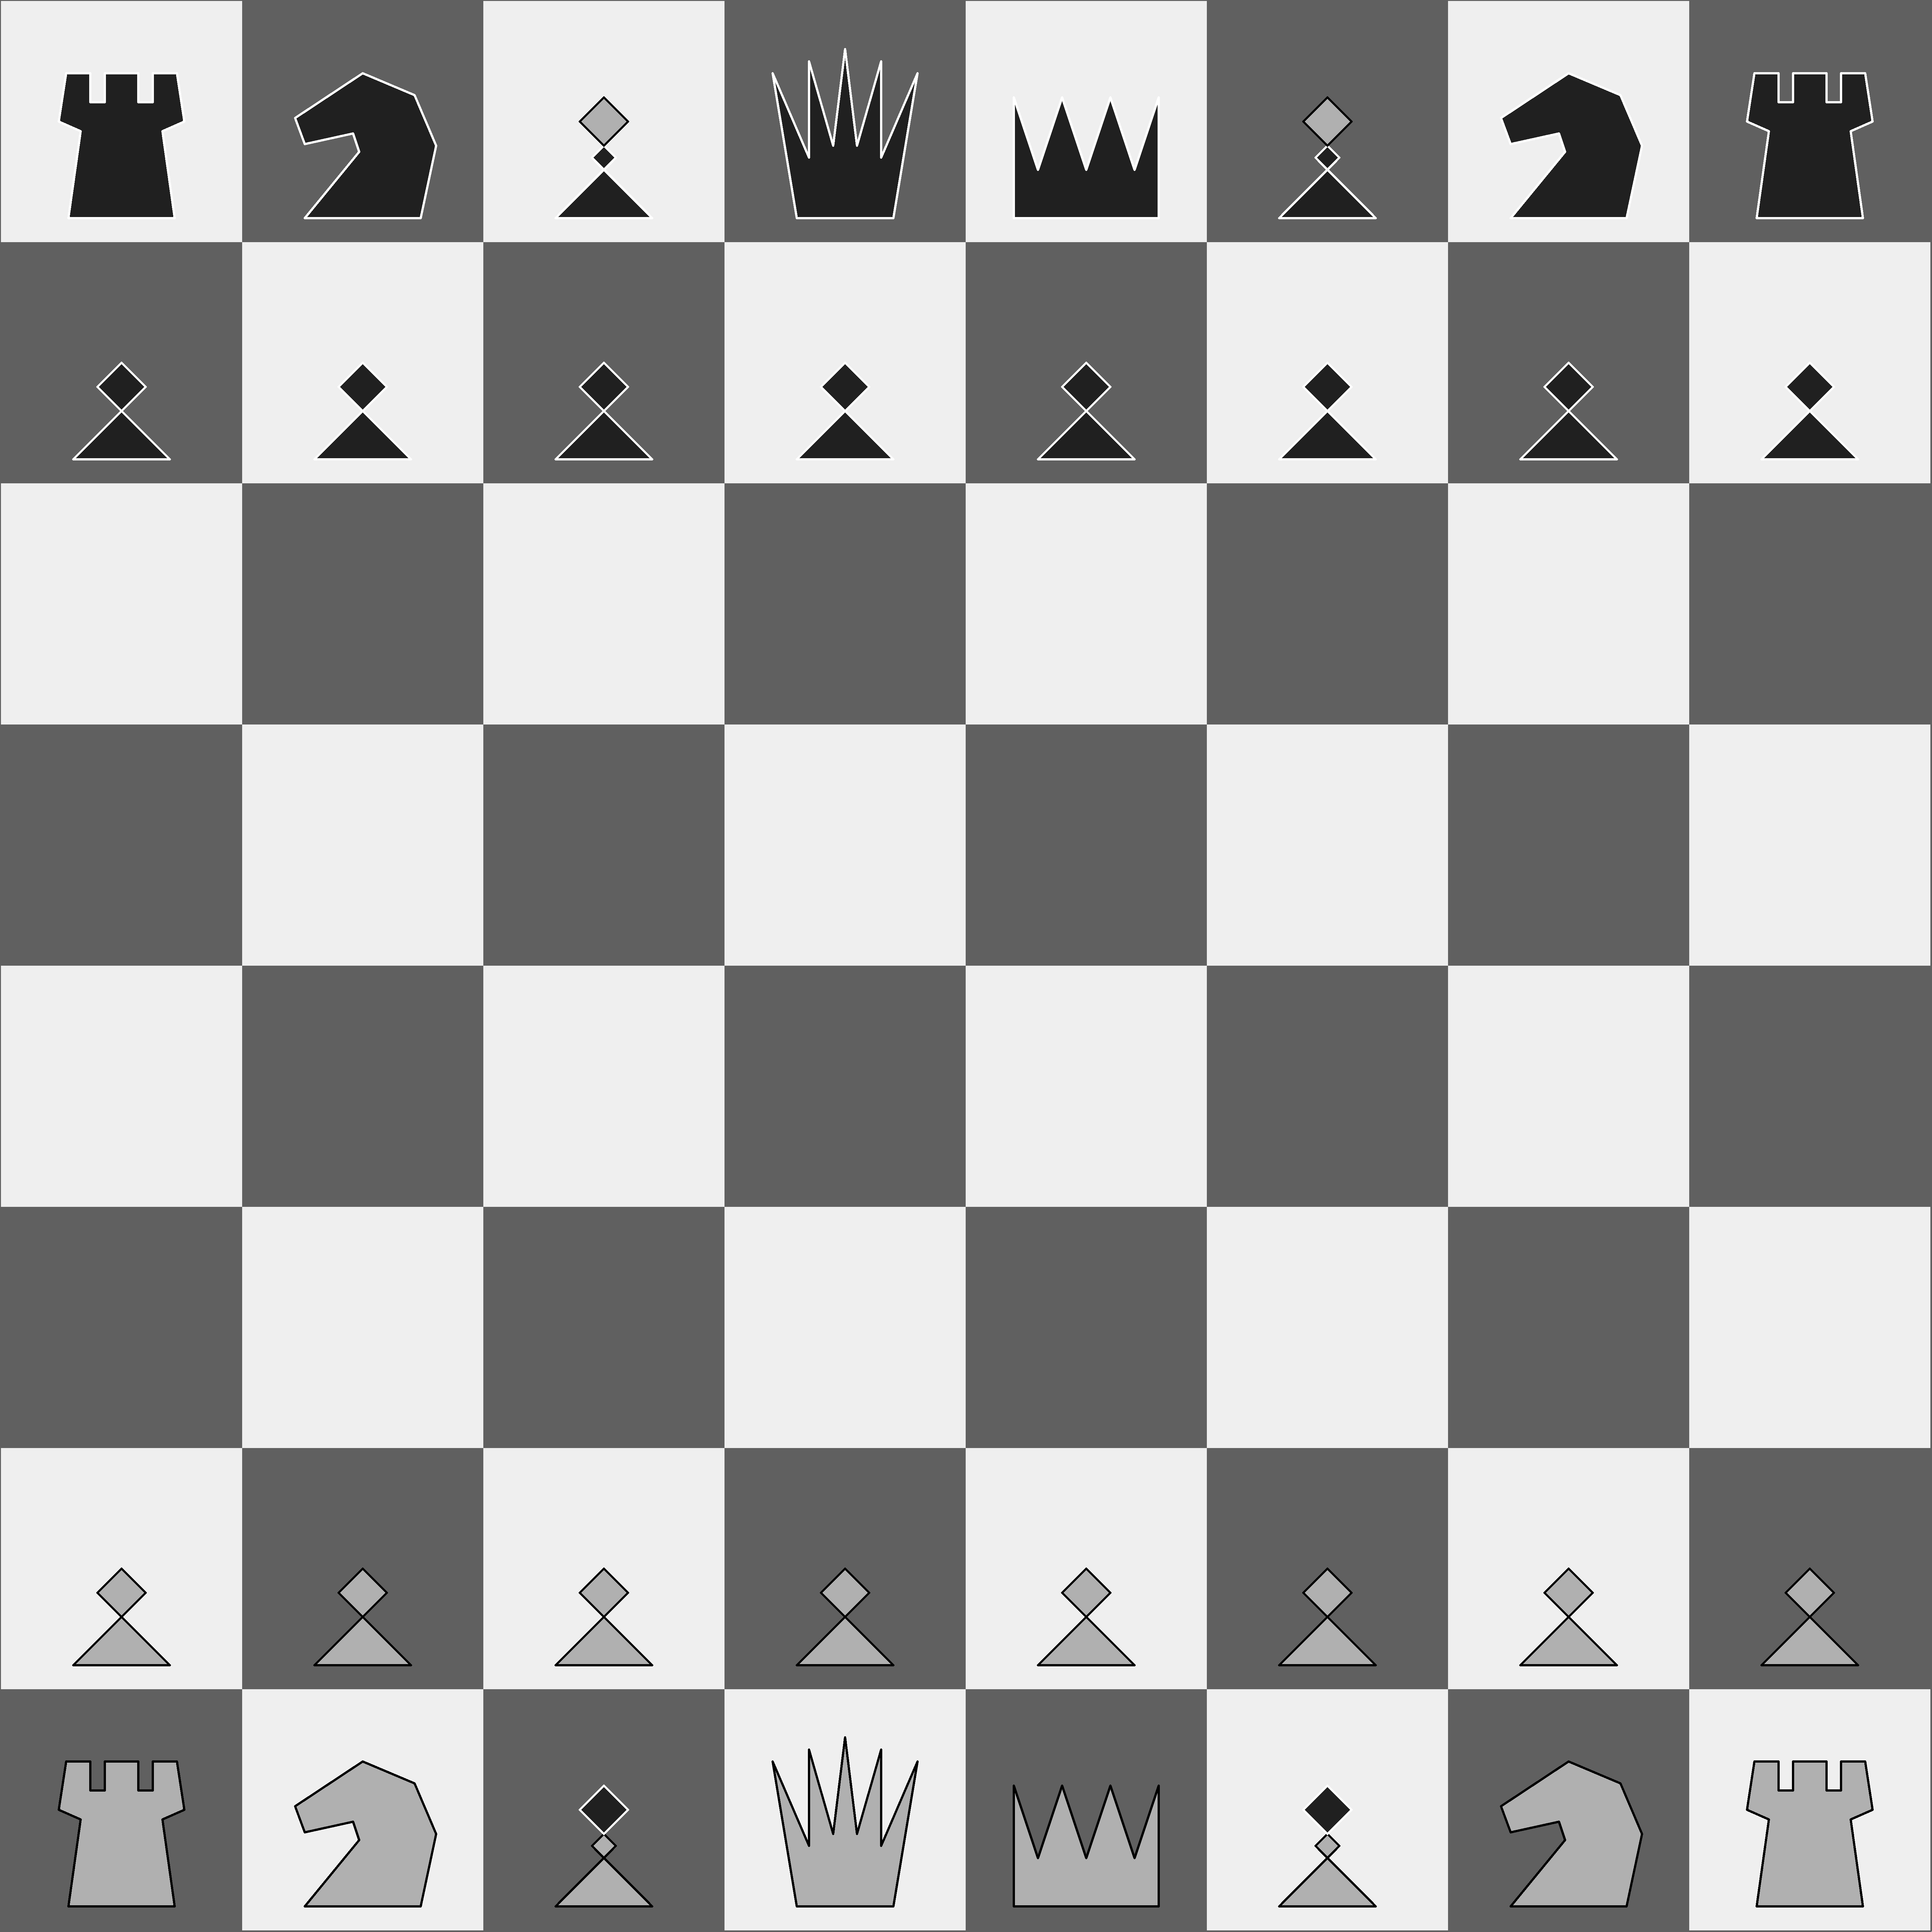
\includegraphics[width=1.0\textwidth, keepaspectratio=true]{boards/02_classical.png}
\caption{Classical board}
\label{fig:classical_chess}
% \centering
\end{figure}

\clearpage
% ---------------------------------------------- Classical Game chapter

